\documentclass[
11pt, % The default document font size, options: 10pt, 11pt, 12pt
%codirector, % Uncomment to add a codirector to the title page
]{charter} 


% El títulos de la memoria, se usa en la carátula y se puede usar el cualquier lugar del documento con el comando \ttitle
\titulo{Construcción de un modelo para predecir la mortalidad en pacientes en diálisis renal} 

% Nombre del posgrado, se usa en la carátula y se puede usar el cualquier lugar del documento con el comando \degreename
\posgrado{Carrera de Especialización en Inteligencia Artificial}

% Tu nombre, se puede usar el cualquier lugar del documento con el comando \authorname
\autor{Lic. Ezequiel Scordamaglia} 

% El nombre del director y co-director, se puede usar el cualquier lugar del documento con el comando \supname y \cosupname y \pertesupname y \pertecosupname
\director{Nombre del Director}
\pertenenciaDirector{pertenencia} 
% FIXME:NO IMPLEMENTADO EL CODIRECTOR ni su pertenencia
%\codirector{John Doe} % para que aparezca en la portada se debe descomentar la opción codirector en el documentclass
\pertenenciaCoDirector{FIUBA}

% Nombre del cliente, quien va a aprobar los resultados del proyecto, se puede usar con el comando \clientename y \empclientename
\cliente{Eugenio Bellia}
\empresaCliente{Grupo DUAM}

% Nombre y pertenencia de los jurados, se pueden usar el cualquier lugar del documento con el comando \jurunoname, \jurdosname y \jurtresname y \perteunoname, \pertedosname y \pertetresname.
\juradoUno{Nombre y Apellido (1)}
\pertenenciaJurUno{pertenencia (1)} 
\juradoDos{Nombre y Apellido (2)}
\pertenenciaJurDos{pertenencia (2)}
\juradoTres{Nombre y Apellido (3)}
\pertenenciaJurTres{pertenencia (3)}
 
\fechaINICIO{17 de octubre de 2023}		%Fecha de inicio de la cursada de GdP \fechaInicioName
\fechaFINALPlan{--------COMPLETAR---------} 	%Fecha de final de cursada de GdP
\fechaFINALTrabajo{--------COMPLETAR---------}	%Fecha de defensa pública del trabajo final


\begin{document}

\maketitle
\thispagestyle{empty}
\pagebreak


\thispagestyle{empty}
{\setlength{\parskip}{0pt}
\tableofcontents{}
}
\pagebreak


\section*{Registros de cambios}
\label{sec:registro}


\begin{table}[ht]
\label{tab:registro}
\centering
\begin{tabularx}{\linewidth}{@{}|c|X|c|@{}}
\hline
\rowcolor[HTML]{C0C0C0} 
Revisión & \multicolumn{1}{c|}{\cellcolor[HTML]{C0C0C0}Detalles de los cambios realizados} & Fecha      \\ \hline
0      & Creación del documento                                 &\fechaInicioName \\ \hline
1      & Se completa hasta el punto 4 inclusive                 & 26 de octubre de 2023 \\ \hline
2      & Se completa hasta el punto 9 inclusive					& 3 de noviembre de 2023 \\ \hline
3      & Se completa hasta el punto 12 inclusive                & 13 de noviembre de 2023 \\ \hline
%		  Se puede agregar algo más \newline
%		  En distintas líneas \newline
%		  Así                                                    & dd/mm/aaaa \\ \hline
%4      & Se completa el plan	                                 & dd/mm/aaaa \\ \hline
\end{tabularx}
\end{table}

\pagebreak



\section*{Acta de constitución del proyecto}
\label{sec:acta}

\begin{flushright}
Buenos Aires, \fechaInicioName
\end{flushright}

\vspace{2cm}

Por medio de la presente se acuerda con el \authorname\hspace{1px} que su Trabajo Final de la \degreename\hspace{1px} se titulará ``\ttitle'', y consistirá en el desarrollo de un modelo predictivo, como prueba piloto, que prediga el nivel de riesgo de mortalidad de un paciente que se encuentre en tratamiento de diálisis renal. Este desarrollo se enmarca en la actualización tecnológica de la organización \empclientename , donde se busca aplicar inteligencia artificial y análisis de datos a nuevos desarrollos que ofrezcan valor agregado a los clientes. El mismo tendrá un presupuesto preliminar estimado de 600 h de trabajo y \$3.864.000, con fecha de inicio \fechaInicioName\hspace{1px} y fecha de presentación pública \fechaFinalName.

Se adjunta a esta acta la planificación inicial.

\vfill

% Esta parte se construye sola con la información que hayan cargado en el preámbulo del documento y no debe modificarla
\begin{table}[ht]
\centering
\begin{tabular}{ccc}
\begin{tabular}[c]{@{}c@{}}Dr. Ing. Ariel Lutenberg \\ Director posgrado FIUBA\end{tabular} & \hspace{2cm} & \begin{tabular}[c]{@{}c@{}}\clientename \\ \empclientename \end{tabular} \vspace{2.5cm} \\ 
\multicolumn{3}{c}{\begin{tabular}[c]{@{}c@{}} \supname \\ Director del Trabajo Final\end{tabular}} \vspace{2.5cm} \\
%\begin{tabular}[c]{@{}c@{}}\jurunoname \\ Jurado del Trabajo Final\end{tabular}     &  & \begin{tabular}[c]{@{}c@{}}\jurdosname\\ Jurado del Trabajo Final\end{tabular}  \vspace{2.5cm}  \\
%\multicolumn{3}{c}{\begin{tabular}[c]{@{}c@{}} \jurtresname\\ Jurado del Trabajo Final\end{tabular}} \vspace{.5cm}                                                                     
\end{tabular}
\end{table}




\section{1. Descripción técnica-conceptual del proyecto a realizar}
\label{sec:descripcion}

Este proyecto, planteado como trabajo final, se realizará para la organización Grupo DUAM, la cual desarrolla software a medida para distintos clientes.
El objetivo principal de este proyecto es incursionar en desarrollos que utilicen las nuevas tecnologías, como son la inteligencia artificial y el análisis de datos, con el fin de proporcionar soluciones innovadoras a problemas preexistentes.
En esta línea, se tomó la decisión de colaborar con uno de sus clientes, una empresa médica que opera centros de atención en todo el país, para crear un primer prototipo que haga uso de estas tecnologías y que, al mismo tiempo, les aporte un valor agregado. Ellos poseen un sistema de gestión de pacientes donde registran datos médicos asociados a cada paciente, como son estudios médicos, hospitalizaciones, medicamentos prescritos, y muchos otros. Es fundamental en la medicina conocer el estado de salud de los pacientes y evaluar los riesgos asociados a ellos. Esto le permite a los profesionales de la salud ajustar el tratamiento y los medicamentos que  prescriben. Pero predecir los riesgos que puede tener un paciente no es tarea sencilla. La complejidad de las condiciones de salud y la gran cantidad de datos clínicos disponibles hacen extremadamente difícil realizar una predicción de mortalidad de manera manual.
En este contexto, surge la idea de ofrecerles desarrollar un modelo predictivo de mortalidad que pueda aprovechar el poder de la inteligencia artificial y del análisis de datos, para realizar un pronóstico rápido y preciso del nivel de riesgo que tiene un paciente.

En este trabajo, se propone partir por la creación de un modelo predictivo de mortalidad que sirva de ejemplo y permita ir desarrollando toda la infraestructura necesaria para que el modelo quede disponible para los usuarios. Se utilizará una plataforma de gestión de modelos y se desarrollará una interfaz por servicio web y un proceso automatizado que solicite las predicciones. Para el desarrollo de este modelo predictivo puntual, se contará con información de miles de pacientes que fueron atendidos por esta empresa médica y sirven de referencia para el proceso de entrenamiento. Se deberán procesar los datos disponibles, entrenar varios modelos de \textit{machine learning} y \textit{deep learning}, evaluar sus métricas y seleccionar los candidatos que logren los mejores resultados.
El desarrollo de este tipo de modelos predictivos, administrados por una plataforma de gestión integral y accesibles por servicio web, permitirá adentrarse en un mercado en constante evolución que demanda soluciones innovadoras. En la figura \ref{fig:diagBloques} se muestra un diagrama de la solución propuesta para resolver el caso piloto.

\begin{figure}[htpb]
\centering 
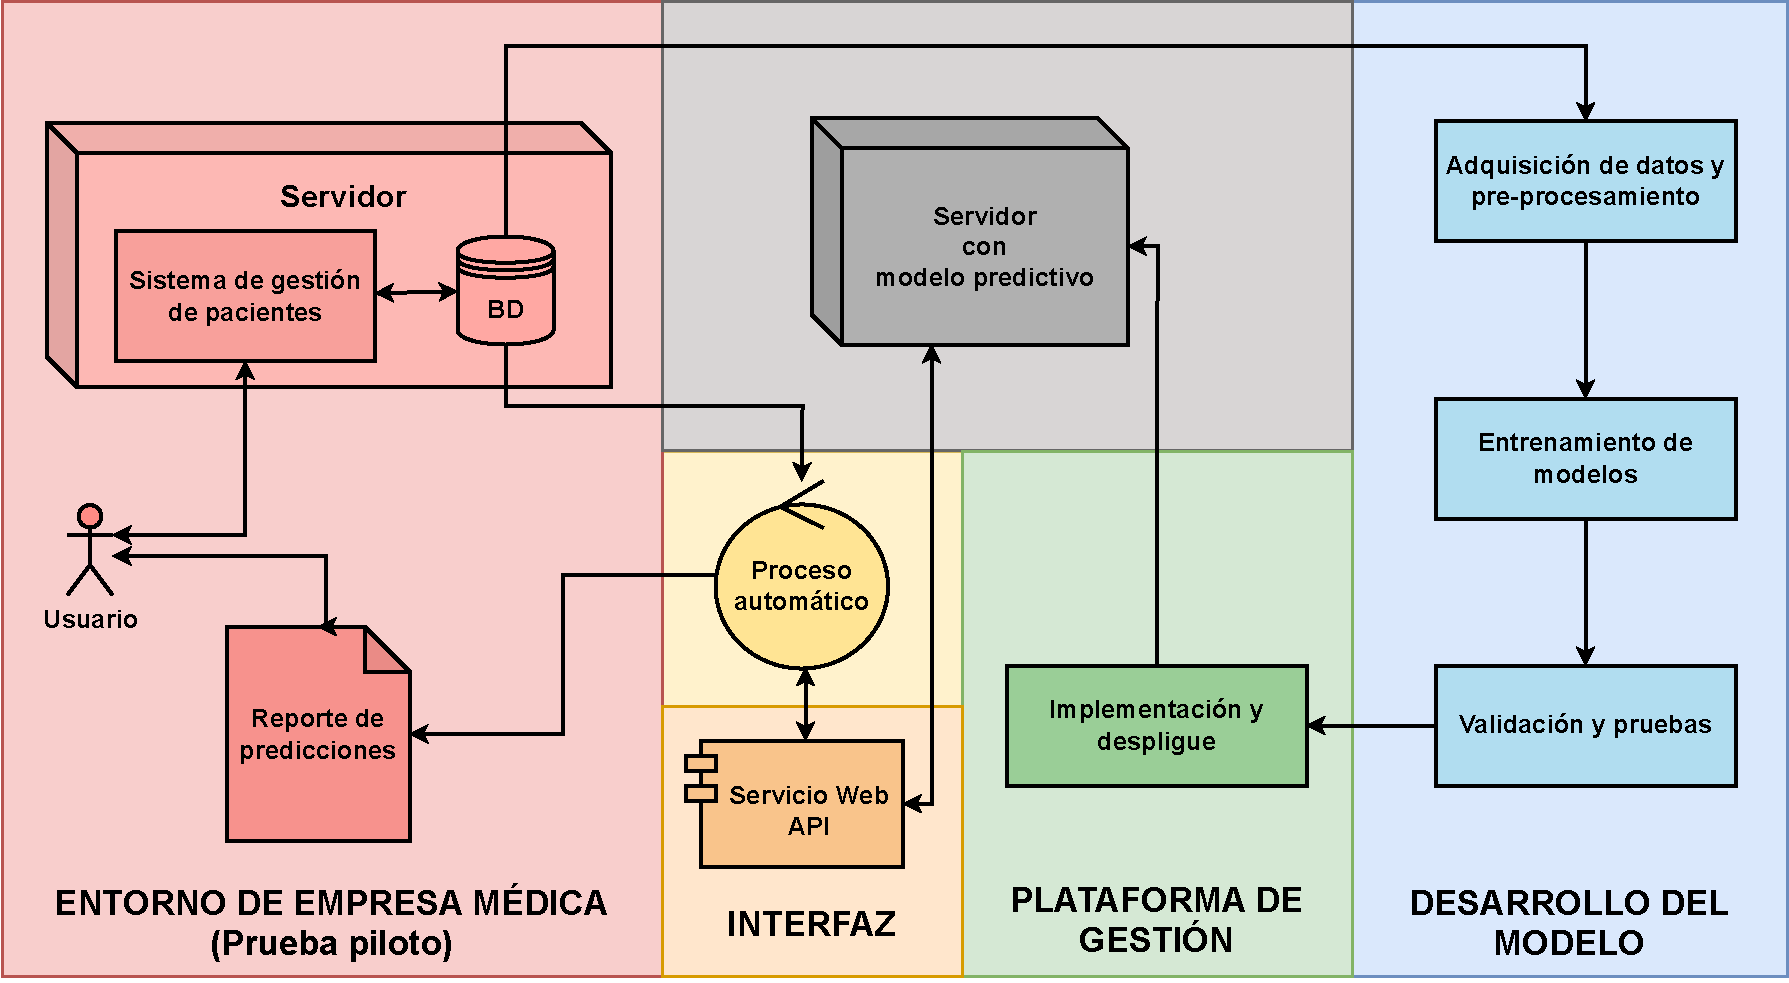
\includegraphics[width=.85\textwidth]{./Figuras/DiagramaDeBloques.pdf}
\caption{Diagrama en bloques del sistema.}
\label{fig:diagBloques}
\end{figure}

Si bien parte del proyecto se limitará a dar solución a un problema puntual en el ámbito médico, el objetivo final es poder brindar soluciones a distintos clientes, incorporando los beneficios de las nuevas tecnologías.
El uso de la inteligencia artificial y el análisis de datos está en auge actualmente, y muchas industrias de distintos campos ya están logrando resultados exitosos. En la medicina ya se han utilizado para la predicción del desarrollo de enfermedades como la diabetes o el cáncer, y también para detectar formas extrañas en imágenes. 
Esto se debe a que los modelos utilizados tienen la capacidad de reconocer patrones en grandes conjuntos de datos.
Para poder generar predicciones es necesario utilizar datos históricos en el entrenamiento, donde los modelos descubren relaciones entre ellos. Luego, por métodos estadísticos, logran predecir eventos futuros basados en dichas relaciones.
Dado que ya se cuenta con los datos históricos de miles de pacientes, este tipo de tecnología podría servir perfectamente para resolver la problemática actual de este cliente. 
El desarrollo de este proyecto tendría dos resultados importantes: dotar a la organización de los conocimientos y herramientas necesarias para resolver problemas que requieran el uso de las nuevas tecnologías, y obtener un producto que resuelva una problemática real, ayudando al personal médico a guiar su trabajo sobre los pacientes más críticos y, en última instancia, salvar vidas.

\section{2. Identificación y análisis de los interesados}
\label{sec:interesados}

\begin{table}[ht]
%\caption{Identificación de los interesados}
%\label{tab:interesados}
\begin{tabularx}{\linewidth}{@{}|l|X|X|l|@{}}
\hline
\rowcolor[HTML]{C0C0C0} 
Rol           & Nombre y Apellido & Organización   & Puesto        \\ \hline
Cliente       & \begin{tabular}[c]{@{}l@{}}\clientename \\ Fabio Rosellini\end{tabular}      & \empclientename & Directores      \\ \hline
Responsable   & \authorname       & FIUBA           & Alumno        \\ \hline
Colaboradores & \begin{tabular}[c]{@{}l@{}}Colaborador 1 \\ Colaborador 2\end{tabular} &  Empresa médica  & \begin{tabular}[c]{@{}l@{}}Gerente de sistemas \\ Asesor de presidencia\end{tabular} \\ \hline
Orientador    & \supname          & \pertesupname    & Director de trabajo final \\ \hline
Usuario final & Personal médico y administrativo   & Empresa médica  & Usuario del sistema   \\ \hline
\end{tabularx}
\end{table}

\begin{itemize}
	\item Cliente: está a favor del desarrollo de este proyecto para impulsar la organización a nuevos mercados y/o ofrecerle desarrollos innovadores a los clientes actuales.
	\item Colaboradores: el asesor de presidencia no tiene mucho tiempo para dedicarle al proyecto, pero puede aportar conocimientos médicos para seleccionar las características más importantes que tengan relación con la mortalidad de los pacientes. Está a favor del desarrollo del proyecto y aportará lo que sea necesario. El gerente de sistemas tampoco tiene mucho tiempo para dedicarle al proyecto, pero es quien dará el permiso para la utilización de los datos. Como no solicitó el desarrollo del proyecto puede que demore en responder si se le consulta algo referido a la infraestructura.
	\item Orientador: puede ayudar mucho en el tratamiento de los datos antes de entrenar los modelos.
	\item Usuario final: necesitará que la predicciones que realiza el modelo estén disponibles en todo momento.
\end{itemize}


\section{3. Propósito del proyecto}
\label{sec:proposito}

El propósito principal de este proyecto es dotar a la organización de nuevas herramientas y capacidades en el ámbito de la inteligencia artificial y el análisis de datos, para poder ofrecer soluciones innovadoras a clientes nuevos o existentes, y poder insertarse en un mercado que se encuentra en constante crecimiento. 

\section{4. Alcance del proyecto}
\label{sec:alcance}

El presente proyecto incluye principalmente la instalación y configuración de una plataforma de gestión de modelos, que permita administrar versiones y ejecutar acciones como el despliegue y el re-entrenamiento de modelos.
Como prueba piloto, se desarrollará un modelo de predicción de mortalidad, que se incorporará a la plataforma de gestión, y también una interfaz que actúe como nexo entre el modelo predictivo y el usuario final.
Para el desarrollo del modelo, se realizarán las tareas de extracción de los datos, su procesamiento, el entrenamiento de los modelos y la evaluación de sus métricas. 
Una vez que se cuente con un modelo entrenado, se realizarán las tareas referidas al despliegue del modelo. 
Con el fin de automatizar la llamada al modelo, se desarrollará también un proceso que envíe automáticamente pedidos de predicciones de todos los pacientes activos cada cierto tiempo al modelo, para que el usuario final cuente con un reporte actualizado en todo momento.
El resultado del modelo podrá ser binario (hay riesgo o no hay riesgo), o categórico, devolviendo un grado de riesgo para ese paciente. Esto se definirá luego de realizar un análisis de los datos disponibles y de los modelos seleccionados para el entrenamiento.

El presente proyecto no incluye el desarrollo de una plataforma de gestión, sino que se elegirá una existente que cumpla con los requerimientos del proyecto. No se desarrollará una interfaz web orientada al usuario final, sino que se desarrollará un servicio web que sea utilizado por procesos automáticos. No se incluirá un proceso de re-entrenamiento automático del modelo.
No se incluye la instalación del modelo predictivo en el entorno productivo de la empresa médica, sino que para el proyecto presentado para este posgrado, se trabajará en un entorno propio de Grupo DUAM que incluirá la plataforma de gestión de modelos, el modelo predictivo y la interfaz por servicio web. Lo único que se instalará en el entorno de la empresa médica será el proceso que recupere datos de los pacientes y llame al servicio web cada cierto período de tiempo para recuperar las predicciones. Esto debe aclararse ya que la instalación en producción de toda la infraestructura no es el objetivo principal de este proyecto, y podría dejarse a cargo del equipo de sistemas de la empresa médica.

\section{5. Supuestos del proyecto}
\label{sec:supuestos}

Para el desarrollo del presente proyecto se supone que:

\begin{itemize}
	\item Se dispone de tiempo en horario laboral para avanzar en el proyecto.
	\item Se dispone de los equipos necesarios para realizar el procesamiento de los datos y el entrenamiento de los modelos.
	\item Se dispone de un ambiente donde poder instalar y configurar la plataforma de gestión, disponibilizar la interfaz por web service y desplegar el modelo para realizar predicciones. 
	\item No hay urgencia en el desarrollo del modelo predictivo.		
	\item Se tiene acceso a los datos médicos de los pacientes.
	\item Se cuenta con un conjunto inicial de datos lo suficientemente grande y representativo para entrenar los modelos de inteligencia artificial de manera efectiva.
	\item Se cuenta con el apoyo de un responsable médico que dé soporte en la selección de variables médicas a utilizar en el entrenamiento de los modelos y también en la interpretación clínica de las predicciones realizadas.
	\item Se mantendrá la protección de datos sensibles de los pacientes y de nuestro cliente en todo momento.		
\end{itemize}

\section{6. Requerimientos}
\label{sec:requerimientos}

\begin{enumerate}
	\item Requerimientos funcionales
		\begin{enumerate}
			\item La plataforma de gestión de modelos deberá permitir desplegar modelos en diversos ambientes.
			\item La interfaz por servicio web deberá recibir datos médicos de uno o varios pacientes y devolver las predicciones asociadas a ellos.			
			\item El modelo predictivo deberá tener una precisión de al menos un 75\%.
			\item El proceso que solicita predicciones y genera el reporte al usuario deberá poder ejecutarse automáticamente cada cierto período de tiempo.		
			\item El reporte de predicciones que le llegue al usuario final deberá tener un formato claro y comprensible.
		\end{enumerate}
	\item Requerimientos de datos a utilizar
		\begin{enumerate}		
		\item Los datos a utilizar para el entrenamiento del modelo deben estar disponibles para los procesos automáticos que re-entrenen al modelo.
		\item Durante el entrenamiento del modelo se deberá resguardar la confidencialidad de los datos de los pacientes.		
		\end{enumerate}
	\item Requerimientos de documentación
		\begin{enumerate}
			\item Redactar una memoria técnica con la información del proyecto.
			\item La documentación de la interfaz por servicio web deberá incluir la lista de métodos disponibles con su detalle.
			\item La documentación del modelo predictivo incluirá información sobre el origen de los datos utilizados para el entrenamiento, las características que se usaron, el detalle del modelo seleccionado y la información que haya sobre la explicabilidad del modelo.
		\end{enumerate}		
\end{enumerate}

\section{7. Historias de usuarios (\textit{Product backlog})}
\label{sec:backlog}

Para poder estimar la cantidad de puntos de historia que representa cada historia de usuario se usarán los siguientes criterios y grados:

\begin{itemize}
	\item Dificultad
	\begin{itemize}
		\item Baja: 1 punto
		\item Media: 3 puntos
		\item Alta: 5 puntos
	\end{itemize}
	\item Complejidad
	\begin{itemize}
		\item Baja: 2 puntos
		\item Media: 5 puntos
		\item Alta: 7 puntos
	\end{itemize}
	\item Incertidumbre
	\begin{itemize}
		\item Baja: 1 punto
		\item Media: 5 puntos
		\item Alta: 10 puntos
	\end{itemize}
\end{itemize}

El puntaje final de cada historia de usuario será calculado como el número de la secuencia de Fibonacci más próximo mayor o igual a la suma de las calificaciones en los 3 criterios.

\begin{itemize}
	\item Como director de la empresa Grupo DUAM, quiero contar con un ambiente en el cual se puedan incluir nuevos modelos predictivos que resuelvan las problemáticas de mis clientes, que sea sencilla y fácil de configurar. (3+5+10 = 18 → 21 puntos)
	\item Como desarrollador de la empresa Grupo DUAM, quiero poder reutilizar los componentes que se desarrollen en proyectos de otros clientes. (3+2+5 = 10 → 13 puntos)
	\item Como médico de centro de la empresa médica, quiero contar con un reporte actualizado de riesgos de mortalidad de los pacientes de mi centro, para poder realizar ajustes en los tratamientos y medicaciones prescritas. (1+5+1 = 7 → 8 puntos)
	\item Como gerente de sistemas de la empresa médica, quiero poder realizar el despliegue del modelo predictivo en producción de manera simple y sencilla. (3+5+1 = 9 → 13 puntos)
\end{itemize}

\section{8. Entregables principales del proyecto}
\label{sec:entregables}

Los entregables del proyecto son:

\begin{itemize}
	\item Documentación del servicio web.
	\item Documentación del modelo predictivo. 
	\item Modelo predictivo de mortalidad.
	\item Plataforma de gestión de modelos correctamente configurada.
	\item Interfaz por servicio web.
	\item Proceso que solicite predicciones y arme un reporte para el usuario de forma automática.
	\item Informe final.
\end{itemize}

\section{9. Desglose del trabajo en tareas}
\label{sec:wbs}

\begin{enumerate}
\item Desarrollo del modelo predictivo de mortalidad (280 h).
	\begin{enumerate}
	\item Investigación sobre variables médicas que tienen influencia en la mortalidad (20 h).
	\item Extracción de datos médicos de la base de datos (40 h).
	\item Procesamiento de datos médicos (40 h).
	\item Entrenamiento de modelos de \textit{machine learning}(40 h).
	\item Entrenamiento de modelos de \textit{deep learning}(40 h).
	\item Evaluación de métricas de los modelos (40 h).
	\item Selección de los modelos candidatos (20 h).
	\item Ajuste fino de los modelos seleccionados (40 h).	
	\end{enumerate}
\item Desarrollo de la interfaz por servicio web (80 h).
	\begin{enumerate}
	\item Diseño de la interfaz (20 h).
	\item Implementación de la interfaz (40 h).
	\item Pruebas sobre la interfaz para obtener predicciones (20 h).	
	\end{enumerate}
\item Instalación y configuración de la plataforma de gestión de modelos (60 h).
	\begin{enumerate}
	\item Investigación de plataformas de gestión de modelos disponibles (10 h).
	\item Instalación de plataforma de gestión seleccionada (30 h).
	\item Configuración de ambientes para despliegue de modelos (20 h).
	\end{enumerate}
\item Desarrollo del proceso automático para solicitar predicciones y generar reportes (80 h).
	\begin{enumerate}
	\item Diseño del proceso que solicita predicciones automáticamente (20 h).
	\item Desarrollo del proceso que solicita predicciones automáticamente (40 h).
	\item Pruebas de automatización de llamadas al modelo (20 h).
	\end{enumerate}
\item Documentación (100 h).
	\begin{enumerate}
	\item Documentación del servicio web (20 h).
	\item Documentación del modelo predictivo (30 h).
	\item Documentación de informe de avance (20 h).
	\item Informe final del proyecto (30 h).
	\end{enumerate}
\end{enumerate}

Cantidad total de horas: 600 h

\section{10. Diagrama de Activity On Node}
\label{sec:AoN}

A continuación, se realiza una breve descripción del Diagrama de Activity On Node que se muestra en la figura \ref{fig:AoN}:

\begin{itemize}
	\item Las tareas de desarrollo del modelo predictivo son las primeras que debe realizarse, ya que de ellas dependen otras actividades como el desarrollo de la interfaz o el desarrollo del proceso automático. 
	\item Las tareas de instalación y configuración de la plataforma de gestión de modelos puede iniciarse junto con el desarrollo del modelo, pero no podrá finalizar hasta que se cuente con el modelo final.
	\item A medida que las tareas de desarrollo vayan finalizado, se documentarán los productos terminados.
\end{itemize}

\begin{figure}[htpb]
\centering 
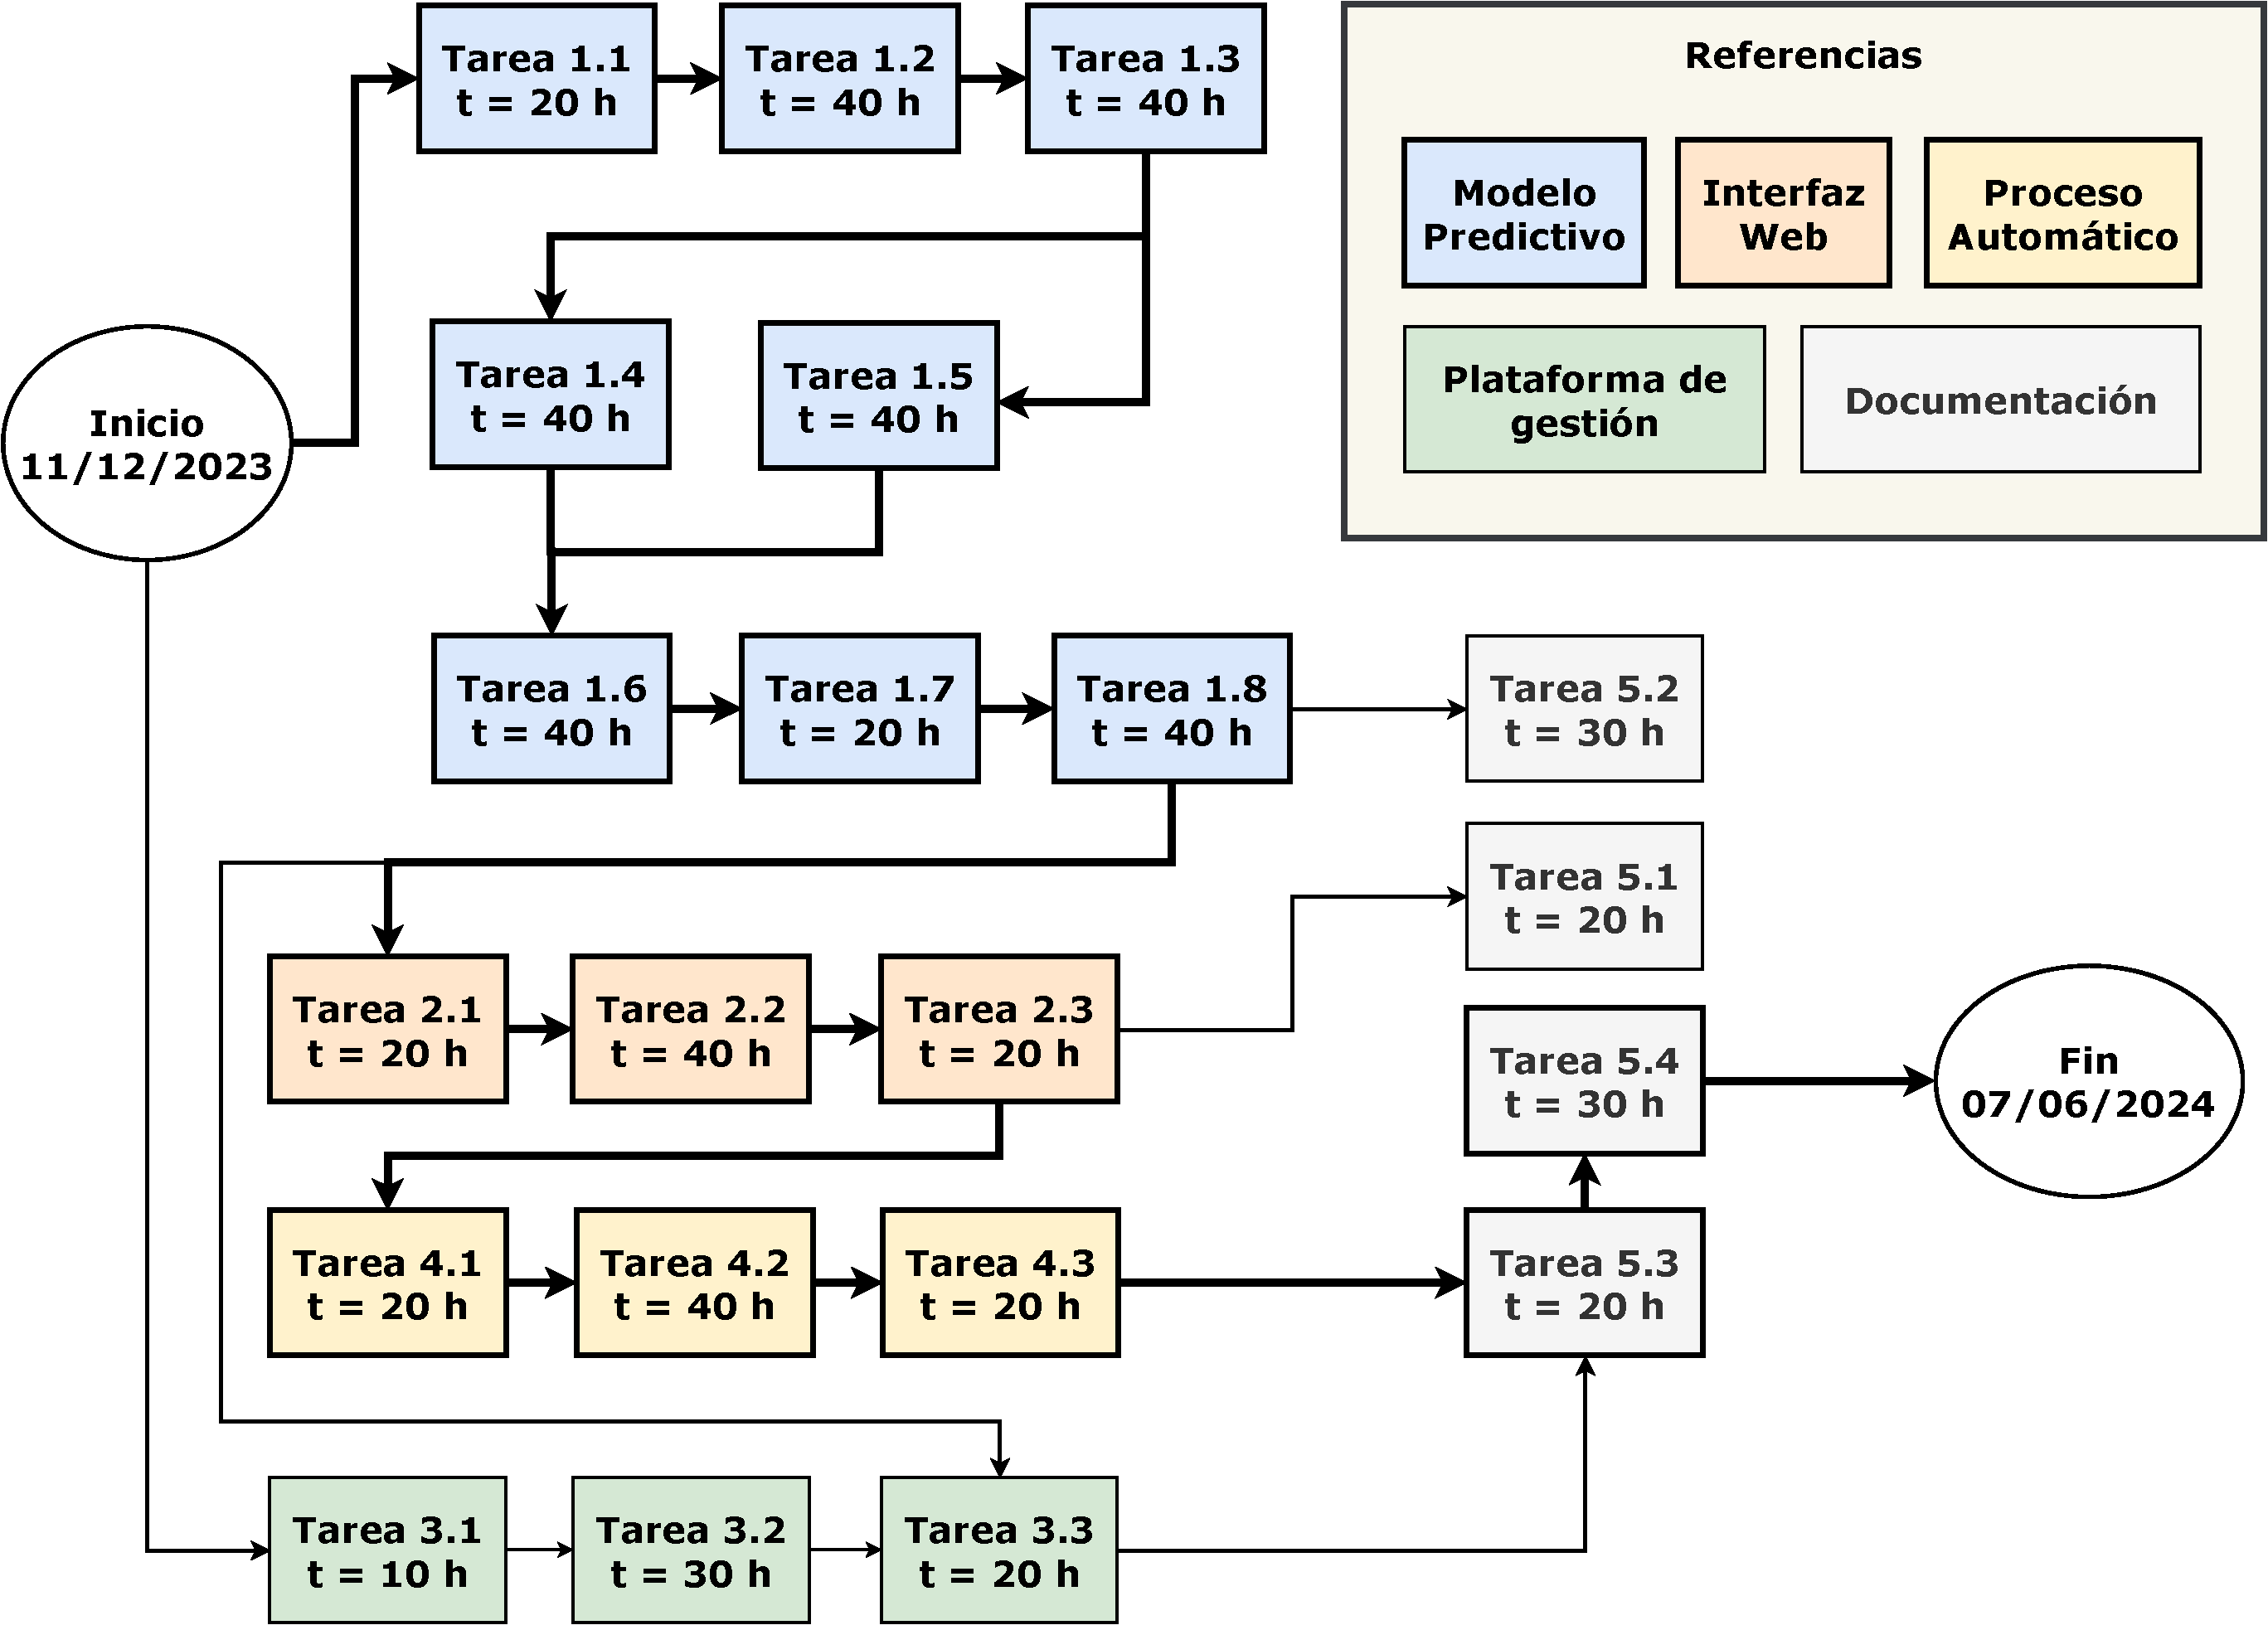
\includegraphics[width=0.99\textwidth]{./Figuras/AoN_Extendido.pdf}
\caption{Diagrama de \textit{Activity on Node} con su camino crítico marcado en negrita}
\label{fig:AoN}
\end{figure}

El camino crítico nos muestra que como mínimo se requieren 450 horas para finalizar el proyecto.


\section{11. Diagrama de Gantt}
\label{sec:gantt}

En la figura \ref{fig:diagGantt01}, se muestra la tabla del Diagrama de Gantt y en la figura \ref{fig:diagGantt02} se muestran las tareas desplegadas sobre la linea de tiempo.

\begin{figure}[htpb]
\centering 
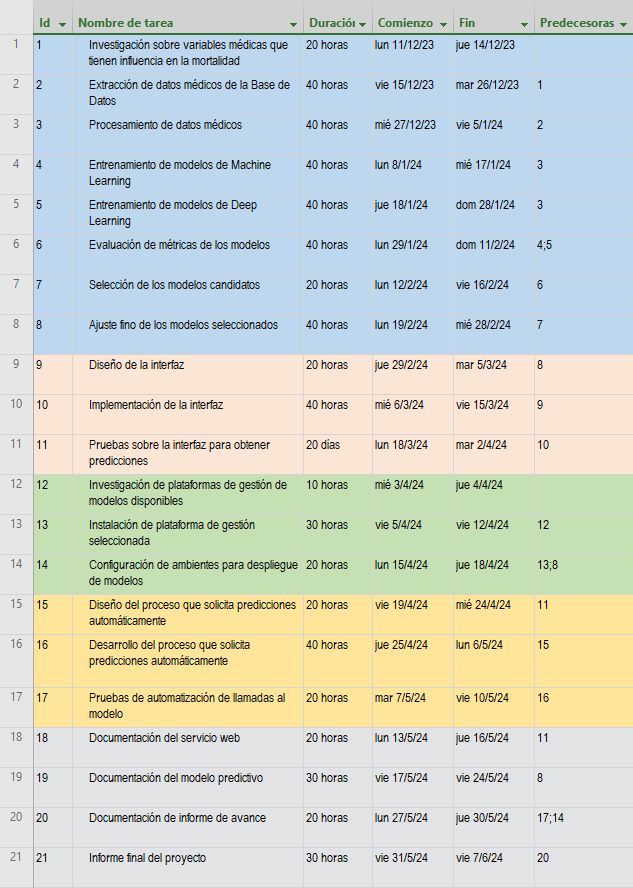
\includegraphics[height=.8\textheight]{./Figuras/Gantt-1.png}
\caption{Tabla del Diagrama de Gantt}
\label{fig:diagGantt01}
\end{figure}


\begin{landscape}
\begin{figure}[htpb]
\centering 
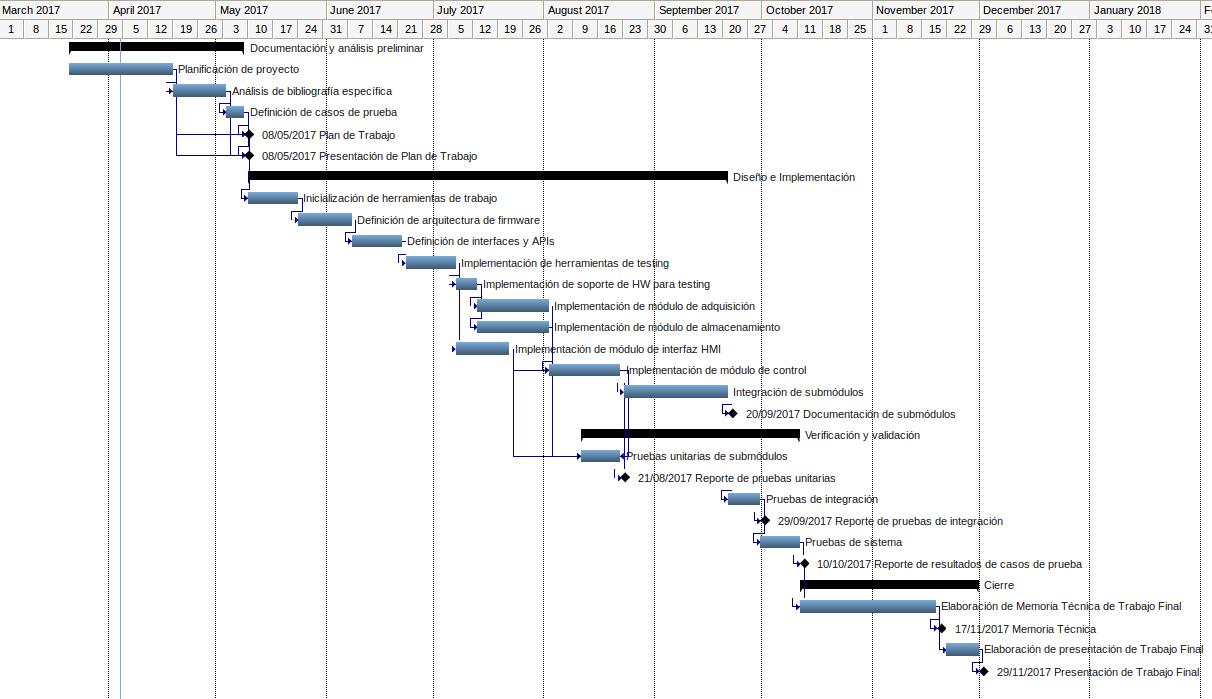
\includegraphics[height=.9\textheight]{./Figuras/Gantt-2.png}
\caption{Diagrama de Gantt}
\label{fig:diagGantt02}
\end{figure}

\end{landscape}

\section{12. Presupuesto detallado del proyecto}
\label{sec:presupuesto}

\begin{table}[htpb]
\centering
\begin{tabularx}{\linewidth}{@{}|X|c|r|r|@{}}
\hline
\rowcolor[HTML]{C0C0C0} 
\multicolumn{4}{|c|}{\cellcolor[HTML]{C0C0C0}COSTOS DIRECTOS} \\ \hline
\rowcolor[HTML]{C0C0C0} 
Descripción &
  \multicolumn{1}{c|}{\cellcolor[HTML]{C0C0C0}Cantidad} &
  \multicolumn{1}{c|}{\cellcolor[HTML]{C0C0C0}Valor unitario} &
  \multicolumn{1}{c|}{\cellcolor[HTML]{C0C0C0}Valor total} \\ \hline
  
 Mano de Obra &
  \multicolumn{1}{c|}{600 h} &
  \multicolumn{1}{c|}{\$4.600/h} &
  \multicolumn{1}{c|}{\$2.760.000} \\ \hline
\multicolumn{3}{|c|}{SUBTOTAL} &
  \multicolumn{1}{c|}{\$2.760.000} \\ \hline
\rowcolor[HTML]{C0C0C0} 
\multicolumn{4}{|c|}{\cellcolor[HTML]{C0C0C0}COSTOS INDIRECTOS} \\ \hline
\rowcolor[HTML]{C0C0C0} 
Descripción &
  \multicolumn{1}{c|}{\cellcolor[HTML]{C0C0C0}Cantidad} &
  \multicolumn{1}{c|}{\cellcolor[HTML]{C0C0C0}Valor unitario} &
  \multicolumn{1}{c|}{\cellcolor[HTML]{C0C0C0}Valor total} \\ \hline
\multicolumn{1}{|l|}{40 \% Costos Indirectos} &
 \multicolumn{1}{c|}{600 h} &
  \multicolumn{1}{c|}{\$1.840/h} &
  \multicolumn{1}{c|}{\$1.104.000} \\ \hline
\multicolumn{3}{|c|}{SUBTOTAL} &
  \multicolumn{1}{c|}{\$1.104.000} \\ \hline
\rowcolor[HTML]{C0C0C0}
\multicolumn{3}{|c|}{TOTAL} & \$3.864.000
   \\ \hline
\end{tabularx}%
\end{table}


\section{13. Gestión de riesgos}
\label{sec:riesgos}

\begin{consigna}{red}
a) Identificación de los riesgos (al menos cinco) y estimación de sus consecuencias:
 
Riesgo 1: detallar el riesgo (riesgo es algo que si ocurre altera los planes previstos de forma negativa)
\begin{itemize}
	\item Severidad (S): mientras más severo, más alto es el número (usar números del 1 al 10).\\
	Justificar el motivo por el cual se asigna determinado número de severidad (S).
	\item Probabilidad de ocurrencia (O): mientras más probable, más alto es el número (usar del 1 al 10).\\
	Justificar el motivo por el cual se asigna determinado número de (O). 
\end{itemize}   

Riesgo 2:
\begin{itemize}
	\item Severidad (S): 
	\item Ocurrencia (O):
\end{itemize}

Riesgo 3:
\begin{itemize}
	\item Severidad (S): 
	\item Ocurrencia (O):
\end{itemize}


b) Tabla de gestión de riesgos:      (El RPN se calcula como RPN=SxO)

\begin{table}[htpb]
\centering
\begin{tabularx}{\linewidth}{@{}|X|c|c|c|c|c|c|@{}}
\hline
\rowcolor[HTML]{C0C0C0} 
Riesgo & S & O & RPN & S* & O* & RPN* \\ \hline
       &   &   &     &    &    &      \\ \hline
       &   &   &     &    &    &      \\ \hline
       &   &   &     &    &    &      \\ \hline
       &   &   &     &    &    &      \\ \hline
       &   &   &     &    &    &      \\ \hline
\end{tabularx}%
\end{table}

Criterio adoptado: 
Se tomarán medidas de mitigación en los riesgos cuyos números de RPN sean mayores a...

Nota: los valores marcados con (*) en la tabla corresponden luego de haber aplicado la mitigación.

c) Plan de mitigación de los riesgos que originalmente excedían el RPN máximo establecido:
 
Riesgo 1: plan de mitigación (si por el RPN fuera necesario elaborar un plan de mitigación).
  Nueva asignación de S y O, con su respectiva justificación:
  - Severidad (S): mientras más severo, más alto es el número (usar números del 1 al 10).
          Justificar el motivo por el cual se asigna determinado número de severidad (S).
  - Probabilidad de ocurrencia (O): mientras más probable, más alto es el número (usar del 1 al 10).
          Justificar el motivo por el cual se asigna determinado número de (O).

Riesgo 2: plan de mitigación (si por el RPN fuera necesario elaborar un plan de mitigación).
 
Riesgo 3: plan de mitigación (si por el RPN fuera necesario elaborar un plan de mitigación).

\end{consigna}


\section{14. Gestión de la calidad}
\label{sec:calidad}

\begin{consigna}{red}
Elija al menos diez requerientos que a su criterio sean los más importantes/críticos/que aportan más valor y para cada uno de ellos indique las acciones de verificación y validación que permitan asegurar su cumplimiento.

\begin{itemize} 
\item Req \#1: copiar acá el requerimiento.

\begin{itemize}
	\item Verificación para confirmar si se cumplió con lo requerido antes de mostrar el sistema al cliente. Detallar 
	\item Validación con el cliente para confirmar que está de acuerdo en que se cumplió con lo requerido. Detallar  
\end{itemize}

\end{itemize}

Tener en cuenta que en este contexto se pueden mencionar simulaciones, cálculos, revisión de hojas de datos, consulta con expertos, mediciones, etc.  Las acciones de verificación suelen considerar al entregable como ``caja blanca'', es decir se conoce en profundidad su funcionamiento interno.  En cambio, las acciones de validación suelen considerar al entregable como ``caja negra'', es decir, que no se conocen los detalles de su funcionamiento interno.

\end{consigna}

\section{15. Procesos de cierre}    
\label{sec:cierre}

\begin{consigna}{red}
Establecer las pautas de trabajo para realizar una reunión final de evaluación del proyecto, tal que contemple las siguientes actividades:

\begin{itemize}
	\item Pautas de trabajo que se seguirán para analizar si se respetó el Plan de Proyecto original:
	 - Indicar quién se ocupará de hacer esto y cuál será el procedimiento a aplicar. 
	\item Identificación de las técnicas y procedimientos útiles e inútiles que se emplearon, y los problemas que surgieron y cómo se solucionaron:
	 - Indicar quién se ocupará de hacer esto y cuál será el procedimiento para dejar registro.
	\item Indicar quién organizará el acto de agradecimiento a todos los interesados, y en especial al equipo de trabajo y colaboradores:
	  - Indicar esto y quién financiará los gastos correspondientes.
\end{itemize}

\end{consigna}


\end{document}
